\documentclass{article}
\usepackage[utf8]{inputenc}
\usepackage{tabularx} % extra features for tabular environment
\usepackage{amsmath}  % improve math presentation
\usepackage{graphicx} % takes care of graphic including machinery
\usepackage{xspace}
\usepackage{tikz}
\usepackage{enumitem}
\usetikzlibrary{babel}
\usepackage[american]{circuitikz}
\usetikzlibrary{calc}
\usepackage{float}
\usepackage{siunitx}
\usepackage{pgfplots}
\usepackage{amsfonts} 
\usetikzlibrary{intersections}
\usepgfplotslibrary{fillbetween}
\usepackage[skins,theorems]{tcolorbox}
\tcbset{highlight math style={enhanced,
  colframe=red,colback=white,arc=0pt,boxrule=1pt}}
\pgfplotsset{width=10cm,compat=1.9}
\usepackage[margin=1in,letterpaper]{geometry} % decreases margins
\usepackage{cite} % takes care of citations
\usepackage[final]{hyperref} % adds hyper links inside the generated PDF file
\hypersetup{
colorlinks=true,       % false: boxed links; true: colored links
linkcolor=blue,        % color of internal links
citecolor=blue,        % color of links to bibliography
filecolor=magenta,     % color of file links
urlcolor=blue        
}

\begin{document}

\title{\textbf{CONVEX OPTIMISATION}\\{\textbf{ASSIGNMENT 1}}}
\author{\textbf{TADIPATRI UDAY KIRAN REDDY}\\\textbf{EE19BTECH11038}}
\maketitle

\section*{\hfil Question 1}
The set \textit{C} can also be represented as,
\begin{equation*}
	C = \{\overline{x}: \mathbf{Y}^T\overline{x} \ge \overline{0}\}
\end{equation*}
Where $\mathbf{Y}$ is a matrix with columns as elements of set $S$.
\subsection*{A: It is not a Subspace.}
Choose $\overline{x_1}, \overline{x_2}$ from set \textit{C}, if this set is subspace then $\forall \alpha _1, \alpha _2 \in \mathbb{R}; \alpha _1\overline{x_1} + \alpha _2\overline{x_2}$ must also be in set \textit{C}.\\
Since $\alpha _1$ and $\alpha _2$ can also take negative value which can the inequatlity, this relation cannot be valid. Thus it is not a Subspace

\subsection*{B: It is not a Affine set.}
The same explanation holds, since the only difference between affine and subspace is that in case of affine $\alpha _1 + \alpha _2 = 1$, but they can take any real values thus can be negative as well. Thus in this case also the ineqality need not satisfy.


\subsection*{C: It is a convex set.}
Choose $\overline{x_1}, \overline{x_2}$ from set \textit{C},
\begin{gather*}
	\mathbf{Y}^T(\theta \overline{x_1}) \ge \overline{0}; \mathbf{Y}^T((1 - \theta )\overline{x_2}) \ge \overline{0}\\
	\implies \mathbf{Y}^T(\theta \overline{x_1} + (1 - \theta )\overline{x_2}) \ge \overline{0}
\end{gather*}
This means that for any $\theta \in [0, 1]$ the above inequality satisfies which means that the set is convex.

\subsection*{D: It is a cone.}
By definition of cone if any set is a cone then any positively scaled vector must also belong to that set.\\
\begin{gather*}
	\mathbf{Y}^T\overline{x} \ge \overline{0}\\
	\implies \mathbf{Y}^T(\theta \overline{x}) \ge \overline{0}; \text{Given } \theta \ge 0
\end{gather*}

Observe that above conditions satisfied despite the nature of matrix $\mathbf{Y}$. Thus we can say that \textbf{none of the above queries depend on structure of \textit{S}}.

\section*{\hfil Question 2}
Given $f_1(\overline{x}) = ||\overline{y}-\mathbf{A}\overline{x}||_2$ and $f_2(\overline(x)) = ||\overline{y}-\mathbf{A}\overline{x}||_2^2$,\\
\begin{list}{•}{\textbf{Useful properties}}
	\item Norm function is convex.
	\item Affine transformation of domain of the function does'nt change the convexity of function.
\end{list}

In case of $f_1(\overline{x})$, the domain is affine transformation of $\overline{x}$ and the norm is operated on it, from above properties the function is convex.\\
\begin{gather*}
	f_1(\overline{x}) = ||\Phi(\overline{x})||_2\\
	\Phi: \overline{x} \rightarrow \overline{y}-\mathbf{A}\overline{x}
\end{gather*}

In case of $f_2(\overline{x})$,
\begin{gather*}
	f_2(\overline{x}) = \overline{x}^T\mathbf{A}^T\mathbf{A}\overline{x} - 2\overline{y}^T\mathbf{A}\overline{x} + \overline{y}^T\overline{y}
\end{gather*}
The above function is quadratic. The function is convex iff $\mathbf{A}^T\mathbf{A}$ is positive semi definite.
\begin{gather*}
	\mathbf{A} = \mathbf{V}\mathbf{\Sigma}\mathbf{V}^T\\
	\implies \mathbf{A}^T\mathbf{A} = (\mathbf{V}\mathbf{\Sigma}\mathbf{V}^T)^T(\mathbf{V}\mathbf{\Sigma}\mathbf{V}^T) = \mathbf{V}\mathbf{\Sigma}^T\mathbf{\Sigma}\mathbf{V}^T
\end{gather*}
$\mathbf{\Sigma}^T\mathbf{\Sigma}$ has positive diagonal entries as above multiplication will yeild individual diagonal entries of $\mathbf{\Sigma}$ to square each other. Since eigen values of $\mathbf{A}^T\mathbf{A}$ are positive thus it is positive definite. Hence $f_2(\overline{x})$ is a convex function.
\section*{\hfil Question 3}
\subsection*{(a)}
Convex hull of $S = \{\overline{x_1}=(0, 0), \overline{x_2}=(1, 1), \overline{x_3}=(1, 0)\}$ is just linear combination of all the vectors such that their coeefficients are positive and they sum up to 1. Since these are 3 non collinear points, which means that convex hull is just the triangle.
\begin{figure}[H]
    \centering


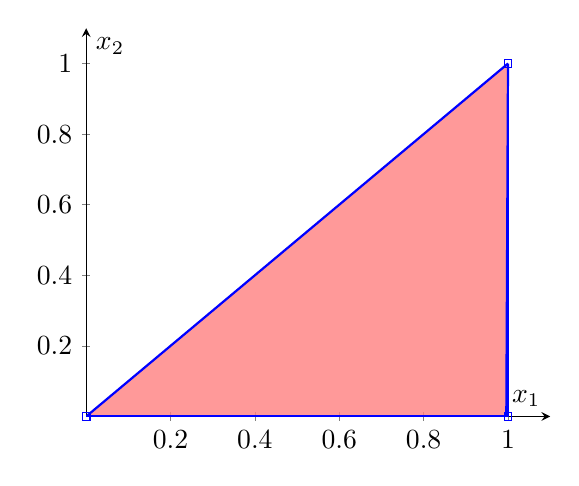
\begin{tikzpicture}[scale=0.7]
    \begin{axis}[
        axis lines=center,
        xmax = 1.1,
        ymax = 1.1,
        ylabel=$x_2$,
        xlabel=$x_1$,
        ]
        \addplot [name path = A,domain=0:1,samples=250,  thick , blue] {x}
            node [pos=0.9, above right] {};
        \addplot [name path = B,domain=0:1,samples=250,  thick , blue] {0*x}
            node [pos=0.1, above right] {};
             \addplot [name path = C,domain=0:1,samples=250,  thick , blue] {x==1}
            node [pos=0.1, above right] {};
        \addplot[red!50, opacity=0.8] fill between[of=A and B];
        \addplot[
    color=blue,
    mark=square,
    ]
    coordinates {
    (0, 0)(1, 0)(1, 1)
    };
        
        
    \end{axis}
\end{tikzpicture}
\caption{conv(\textit{S})}
\end{figure}
\subsection*{(b)}
Take a point inside convex hull,
\begin{figure}[H]
    \centering


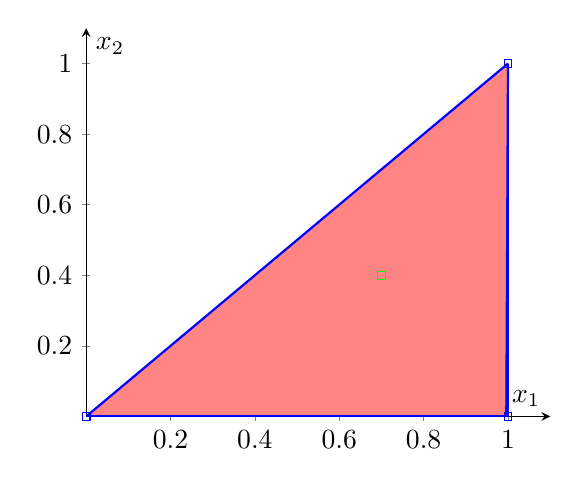
\begin{tikzpicture}[scale=0.7]
    \begin{axis}[
        axis lines=center,
        xmax = 1.1,
        ymax = 1.1,
        ylabel=$x_2$,
        xlabel=$x_1$,
        ]
        \addplot [name path = A,domain=0:1,samples=250,  thick , blue] {x}
            node [pos=0.9, above right] {};
        \addplot [name path = B,domain=0:1,samples=250,  thick , blue] {0*x}
            node [pos=0.1, above right] {};
             \addplot [name path = C,domain=0:1,samples=250,  thick , blue] {x==1}
            node [pos=0.1, above right] {};
        \addplot[red!50, opacity=0.8] fill between[of=A and B];
        \addplot[red!50, opacity=0.8] fill between[of=A and B];
        \addplot[
    color=blue,
    mark=square,
    ]
    coordinates {
    (0, 0)(1, 0)(1, 1)
    };
        \addplot[
    color=green,
    mark=square,
    ]
    coordinates {
    (0.7, 0.4)}
     ;
        
        
    \end{axis}
\end{tikzpicture}
\end{figure}
This point can be written as $\overline{v}=\sum_{i=1}^{3}{\theta _i}\overline{x_i}$ such that $\sum_{i=1}^{3}{\theta _i} = 1$. Given f is convex function which means that,\\
\begin{gather*}
	f(\overline{v}) = f(\sum_{i=1}^{3}{\theta _i}\overline{x_i})\\
	\implies f(\overline{v}) \le \sum_{i=1}^{3}{\theta _i}f(\overline{x_i})
	f(\overline{v}) \le \sum_{i=1}^{3}{\theta _i}max\{f(\overline{x_i})\} = max\{f(\overline{x_i})\}\sum_{i=1}^{3}{\theta _i}\\
	\implies f(\overline{v}) \le max\{f(\overline{x_i})\}
\end{gather*}
Clearly from above inequalities we see that value of any point in convex hull of polyhedra is always less than equal to the value of maximum value at vertices given \textit{f} is convex, which means maxima occurs at vertices.
\section*{\hfil Question 4}
\section*{\hfil Question 5}
\subsection*{(a)}
Let $\overline{x}^*$ be one of the optimum solution to the the function $f$ on set convex set $C$. Further it is given that bot function $f$ and set $C$ are symmentric convex.\\
If $\overline{x}^* = \begin{pmatrix} x_1^* \\ x_2^* \end{pmatrix}$ is a solution then the following vector is also a solution $\tilde{\overline{x}} = \begin{pmatrix} x_2^* \\ x_1^* \end{pmatrix}$ since the function is symmentric $f(\overline{x}) = f(\tilde{\overline{x}})$.\\
By convex nature of the function,\\
\begin{gather*}
	f(\alpha\overline{x}^* + (1-\alpha)\tilde{\overline{x}}) \le \alpha f(\overline{x}^*) + (1-\alpha)f(\tilde{\overline{x}})\\
	\implies f(\alpha\overline{x}^* + (1-\alpha)\tilde{\overline{x}}) \le f(\overline{x}) = f(\tilde{\overline{x}}) = min_{\overline{x} \in C}\{f(\overline{x})\} \\ 
	\implies f(\alpha\overline{x}^* + (1-\alpha)\tilde{\overline{x}}) = min_{\overline{x} \in C}\{f(\overline{x})\}
\end{gather*}
This means that any point on line joining the points $\overline{x}^*$ and $\tilde{\overline{x}}$ is a solution the optimisation problem.\\
Setting $\alpha = 0.5$, $\overline{a} = \frac{\overline{x}^* + \tilde{\overline{x}}}{2} = \begin{pmatrix} \frac{x_1^* + x_2^*}{2} \\ \frac{x_2^* + x_1^*}{2} \end{pmatrix}$. Now observe that obtained $\overline{a}$ has equal coordinates. Thus there exists an optimum $\overline{x}$ with both coordinates equal.
\subsection*{(b)}
\textbf{AM-GM Inequality}\\
Given $x_i \ge 0$,
\begin{equation*}
	\frac{1}{N}\sum_{i=1}^{N}x_i \ge \sqrt[N]{\Pi _{i=1}^{N}x_i}
\end{equation*}
We can solve the given optimisation problem using above inequality.\\
\begin{gather*}
	\sqrt[n]{x_1x_2x_3...x_n} \le \frac{1}{n}\sum_{i=1}^{n}x_i = \frac{1}{n}\\
	\implies x_1x_2x_3...x_n \le \frac{1}{n^n}
\end{gather*}
Therefore, optimal value is $\frac{1}{n^n}$.
\section*{\hfil Question 6}
\subsection*{(a)}
Let $g(\overline{x}) = \overline{x}^T\overline{x}$ then $f(\overline{x}, t)$ can be written as $tg(\frac{\overline{x}}{t})$. Now we look at the epigraph of $f$.
\begin{gather*}
	epi(f) = \left\{\begin{pmatrix}
	\overline{x}\\
	t\\
	z
	\end{pmatrix} : t > 0; z \ge f(\overline{x}, t)\right\}\\
	epi(f) = \left\{\begin{pmatrix}
	\overline{x}\\
	t\\
	z
	\end{pmatrix} : t > 0; z \ge tg\left(\frac{\overline{x}}{t}\right)\right\} = \left\{\begin{pmatrix}
	\overline{x}\\
	z\\
	t
	\end{pmatrix} : t > 0; \frac{z}{t} \ge g\left(\frac{\overline{x}}{t}\right)\right\}
\end{gather*}
Now let us look at perspective of $epi(f)$,
\begin{gather*}
perspctive(epi(f)) = \left\{\begin{pmatrix}
	\overline{x}/t\\
	z/t
	\end{pmatrix} : t > 0; \frac{z}{t} \ge g\left(\frac{\overline{x}}{t}\right)\right\}
\end{gather*}

We know that $g$ is convex as it is a quadratic function with positive definite hessian matrix. And above set is nothing but epigraph of $g$ thus it is also convex. Now since epigraph of $g$ is convex and it is same as perspective of epigraph of $f$. This implies that epigraph of $f$ is also convex. Thus we can conclude that $f$ is also convex as it's epigraph is convex.
\subsection*{(b)}
If function $f$ is quasi convex then it's domain and all its $\alpha$-sublevel sets are convex are called as "Quasi-convex".\\
Consider the below $\alpha$-sublevel set,
\begin{gather*}
	S_{\alpha} = \left\{\begin{pmatrix}
	\overline{x}\\
	t
	\end{pmatrix}: \frac{\overline{x}^T\overline{x}}{t^2} \le \alpha \right\}
\end{gather*}
\subsection*{(c)}
Let $\tilde{\overline{x}} = \frac{\overline{x}}{||\overline{x}||_2}$ then,
\begin{equation*}
	f(\overline{x}) = \begin{cases}
	||\overline{x}||_2 - 1 & if||x||_2 \ge 1\\
	0 & otherwise
	\end{cases}
\end{equation*}
We can rewrite the equation as,
\begin{equation*}
	f(\overline{x}) = max\{||\overline{x}||_2 - 1, 0\}
\end{equation*}
We know that max of convex functions is convex, $||x||_2-1$ is convex since it is just norm function but with a bias and 0 is trivially convex. Thus $f$ is convex.
\end{document}